

%\begin{figure}
%    \centering
%    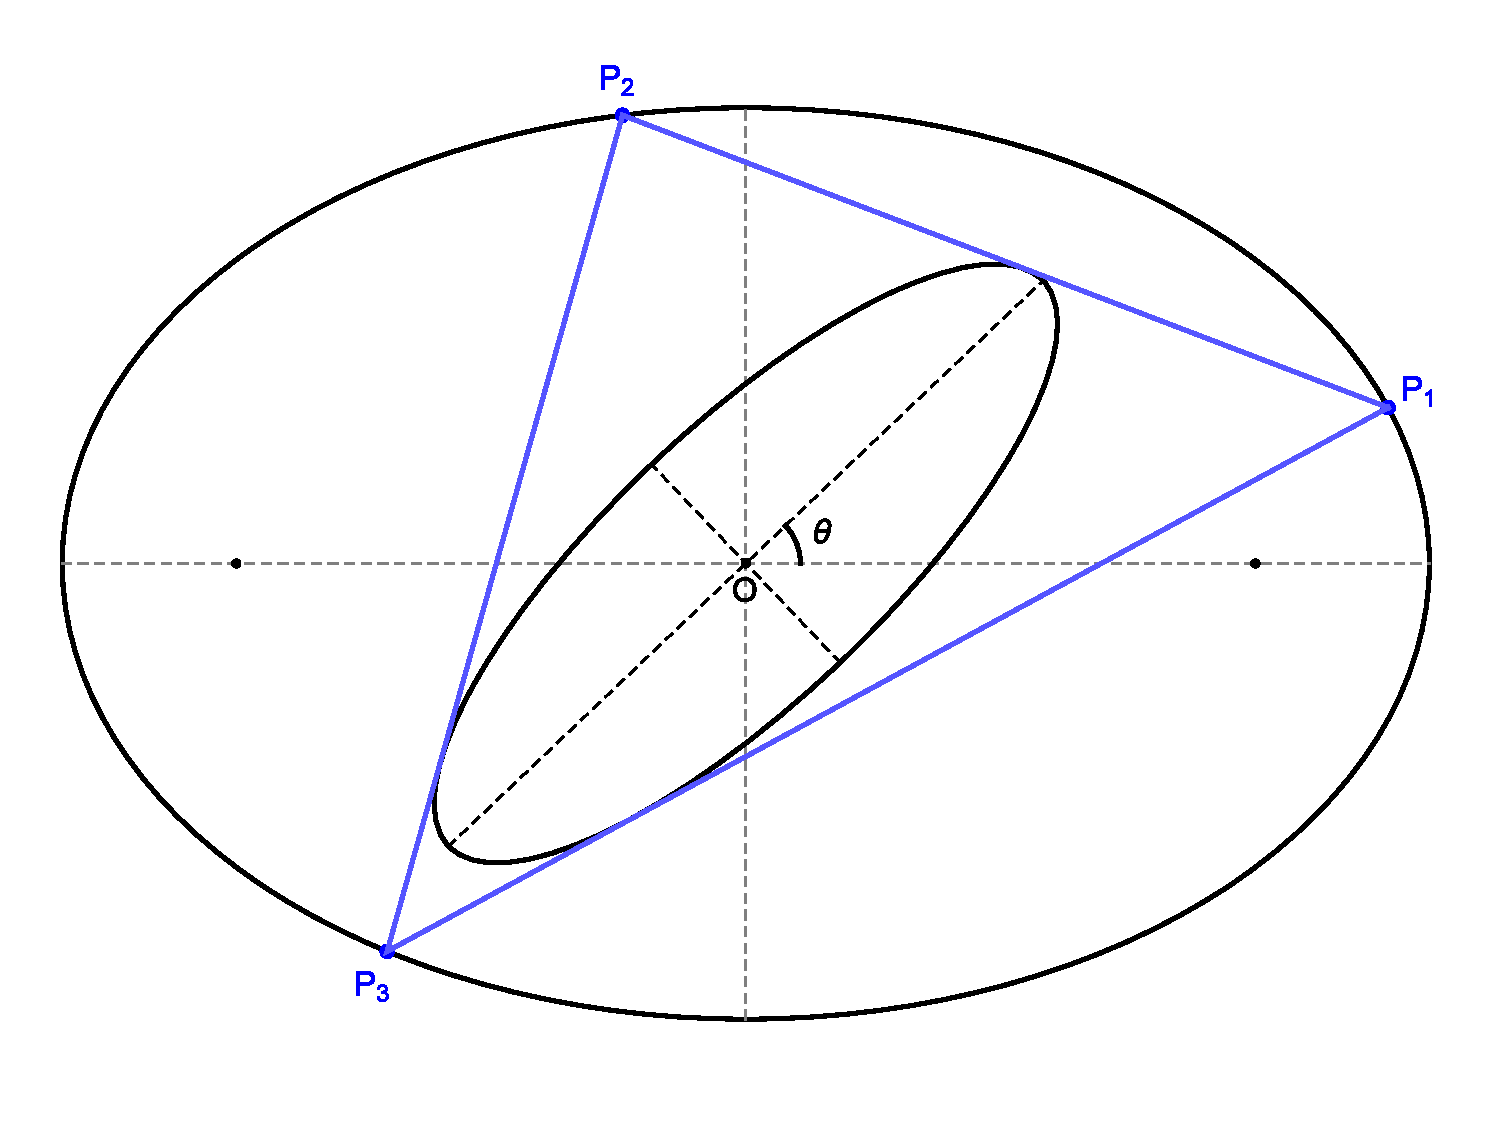
\includegraphics[width=.7\textwidth]{pics/0020_n3_tilted.eps}
%    \caption{A concentric, unaligned pair of ellipses which admits a 3-periodic family (blue). Their major axes are tilted by $\theta$.}
%    \label{fig:n3-tilted}
%\end{figure}

Consider two nested ellipses $\E$ and $\E_c$ with semi-axes $(a,b)$ and $(a_c,b_c)$: $\E$ is centered at the origin $O$ and $\E_c$ at $O_c=(x_c,y_c)$. Let $\theta$ denote the angle between their major axes; see Figure~\ref{fig:n3-general-pos}. If $O_c=0$ we call the pair ``concentric''. If $\theta=0$ we call it ``axis-aligned''. Additionally, let $c^2={a^2-b^2}$ and $c_c^2={a_c^2-b_c^2}$ denote their half focal distances. Note these are the squares of half the focal distance.

\begin{definition}
The power $\P_X$ of a point $X$ with respect to a circle centered on $C$ and of radius $R$ is given by \cite[Circle Power]{mw}:

\[ \P_X(C,R) = |X-C|^2-R^2 \]
\end{definition}

Recall the circumcircle passes through triangle vertices. Using Kimberling's notation for triangle centers \cite{etc}, let $X_3$ and $R$ denote its center and radius; these are known as circumcenter and circumradius. Also recall Euler's (or Feuerbach's, or the 9-point) circle: it passes through the sides' midpoints. Its radius is half the circumradius \cite[Nine-point circle]{mw}. Let $X_5$ denote its center. The following shorthands will be used for the power of a point $O$ wrt to either circumcircle or Euler's circle:

\[ \P_3 = \P_{O}(X_3,R),\;\;\;\P_5 = \P_{O}(X_5,R/2) \]
